\documentclass[tikz,border=0pt]{standalone}

\usepackage[T1]{fontenc}
\usepackage[american]{circuitikz}
\usetikzlibrary{arrows.meta,backgrounds,calc,fit}

\definecolor{MainBus}{HTML}{9C2F24}
\definecolor{SenseWire}{HTML}{1769AA}
\definecolor{SdaWire}{HTML}{00838F}
\definecolor{SclWire}{HTML}{6A4C93}
\definecolor{LogicPower}{HTML}{B05A00}
\definecolor{ModuleFill}{HTML}{F4F7FA}
\definecolor{WarningRed}{HTML}{B3261E}
\definecolor{ChargeGreen}{HTML}{18794E}
\definecolor{DischargeOrange}{HTML}{B54708}

\tikzset{
  module body/.style={
    draw=black!75,
    fill=ModuleFill,
    line width=0.9pt,
    rounded corners=2pt,
    inner sep=0pt
  },
  module title/.style={
    font=\sffamily\bfseries,
    align=center
  },
  module port/.style={
    circle,
    draw=black!70,
    line width=0.5pt,
    minimum size=5pt,
    inner sep=0pt
  },
  port label/.style={
    font=\sffamily\tiny\bfseries,
    text=black!80,
    inner sep=0.7pt
  },
  main current/.style={draw=MainBus, line width=2.3pt},
  sense/.style={draw=SenseWire, line width=1.0pt},
  i2c cable/.style={draw=black!35, line width=6.0pt, line cap=round},
  sda/.style={draw=SdaWire, line width=1.35pt, line cap=round},
  scl/.style={draw=SclWire, line width=1.35pt, line cap=round},
  logic power/.style={draw=LogicPower, line width=1.0pt},
  note/.style={font=\sffamily\scriptsize, align=center},
  label text/.style={font=\sffamily\small, align=center},
  warning box/.style={
    draw=WarningRed,
    fill=WarningRed!5,
    text=WarningRed,
    line width=0.8pt,
    rounded corners=2pt,
    font=\sffamily\scriptsize\bfseries,
    align=center,
    inner sep=4pt
  },
  pics/module/.style args={#1/#2/#3}{
    code={
      \node[module body, minimum width=#2, minimum height=#3] (-body) {};
      \node[module title, anchor=north, yshift=-6pt] at (-body.north) {#1};
    }
  }
}

% A named electrical port on a module boundary. Arguments are node name,
% coordinate, visible label, label direction, and net color.
\newcommand{\ModulePort}[5]{%
  \node[module port, fill=#5, label={[port label]#4:{#3}}] (#1) at #2 {};%
}

\ctikzset{
  bipoles/thickness=1.4,
  nodes width=0.08
}

\begin{document}
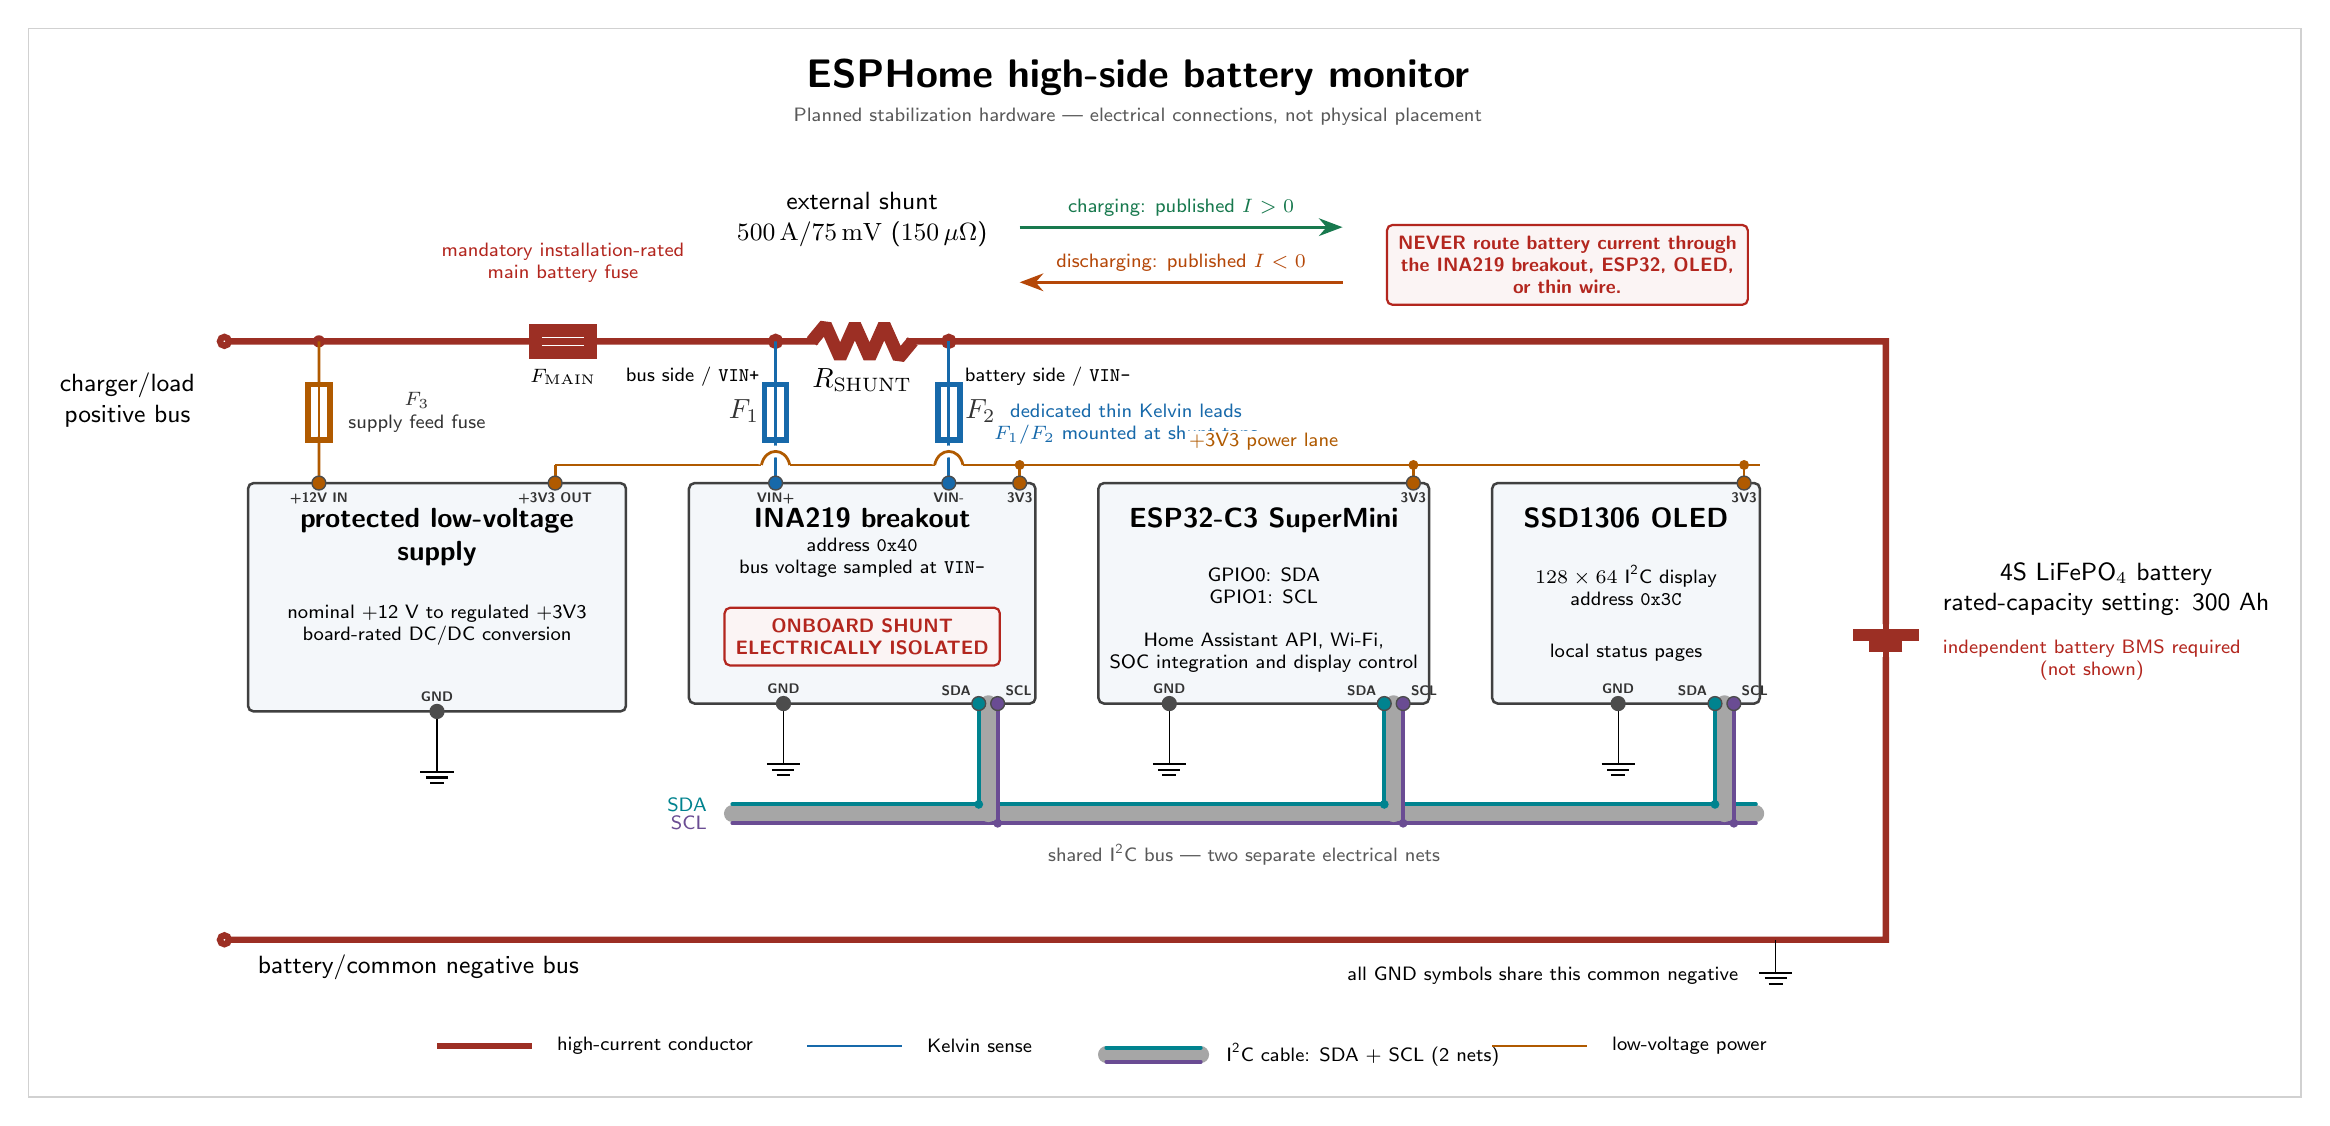
\begin{tikzpicture}[font=\sffamily]
  \begin{scope}[local bounding box=diagram-content]

  % --------------------------------------------------------------------------
  % Title
  % --------------------------------------------------------------------------
  \node[font=\sffamily\Large\bfseries] at (9.5,10.35)
    {ESPHome high-side battery monitor};
  \node[note, text=black!65] at (9.5,9.85)
    {Planned stabilization hardware --- electrical connections, not physical placement};

  % --------------------------------------------------------------------------
  % High-current path. Main current must never enter the INA219 breakout.
  % --------------------------------------------------------------------------
  \draw[main current]
    (-2.1,7.0) to[short, o-] (1.0,7.0)
    to[fuse] (3.4,7.0)
    -- (4.9,7.0)
    to[R, l_={$R_{\mathrm{SHUNT}}$}, *-*] (7.1,7.0)
    -- (19.0,7.0)
    to[battery1] (19.0,-0.6)
    -- (-1.8,-0.6) to[short, -o] (-2.1,-0.6);

  \node[label text, anchor=north east] at (-2.35,6.72)
    {charger/load\\positive bus};
  \node[note, text=WarningRed] at (2.2,8.0)
    {mandatory installation-rated\\main battery fuse};
  \node[note] at (2.2,6.55) {$F_{\mathrm{MAIN}}$};
  \node[label text] at (6.0,8.55)
    {external shunt\\$500\,\mathrm{A}/75\,\mathrm{mV}$ ($150\,\mu\Omega$)};
  \node[note, anchor=east] at (4.82,6.55) {bus side / \texttt{VIN+}};
  \node[note, anchor=west] at (7.18,6.55) {battery side / \texttt{VIN-}};

  \draw[draw=ChargeGreen, line width=1.0pt, -{Stealth[length=3mm]}]
    (8.0,8.45) -- (12.1,8.45)
    node[midway, above, note, text=ChargeGreen] {charging: published $I>0$};
  \draw[draw=DischargeOrange, line width=1.0pt, -{Stealth[length=3mm]}]
    (12.1,7.75) -- (8.0,7.75)
    node[midway, above, note, text=DischargeOrange] {discharging: published $I<0$};
  \node[warning box, anchor=south west] at (12.65,7.45)
    {NEVER route battery current through\\the INA219 breakout, ESP32, OLED,\\or thin wire.};

  \node[label text, anchor=west] at (19.6,3.85)
    {4S LiFePO$_4$ battery\\rated-capacity setting: 300 Ah};
  \node[note, anchor=west, text=WarningRed] at (19.6,2.95)
    {independent battery BMS required\\(not shown)};
  \node[label text, anchor=west] at (-1.8,-0.95)
    {battery/common negative bus};
  \draw (17.6,-0.6) node[ground] {};
  \node[note, anchor=east] at (17.25,-1.05)
    {all GND symbols share this common negative};

  % --------------------------------------------------------------------------
  % Fused, dedicated Kelvin leads from the two external-shunt sense points.
  % --------------------------------------------------------------------------
  \draw[sense]
    (4.9,7.0) to[fuse, l_={\textcolor{black!80}{$F_1$}}] (4.9,5.2);
  \draw[sense]
    (7.1,7.0) to[fuse, l={\textcolor{black!80}{$F_2$}}] (7.1,5.2);
  \node[note, text=SenseWire, anchor=west] at (7.55,5.95)
    {dedicated thin Kelvin leads\\$F_1/F_2$ mounted at shunt taps};

  % --------------------------------------------------------------------------
  % INA219 breakout with its onboard differential shunt isolated.
  % --------------------------------------------------------------------------
  \pic (ina219) at (6.0,3.8)
    {module={INA219 breakout/4.4cm/2.8cm}};
  \node[note] at (6.0,4.25)
    {address \texttt{0x40}\\bus voltage sampled at \texttt{VIN-}};
  \node[warning box] at (6.0,3.25)
    {ONBOARD SHUNT\\ELECTRICALLY ISOLATED};

  % --------------------------------------------------------------------------
  % Controller and display modules.
  % --------------------------------------------------------------------------
  \pic (esp32) at (11.1,3.8)
    {module={ESP32-C3 SuperMini/4.2cm/2.8cm}};
  \node[note] at (11.1,3.9)
    {GPIO0: SDA\\GPIO1: SCL};
  \node[note] at (11.1,3.05)
    {Home Assistant API, Wi-Fi,\\SOC integration and display control};

  \pic (oled) at (15.7,3.8)
    {module={SSD1306 OLED/3.4cm/2.8cm}};
  \node[note] at (15.7,3.9)
    {$128\times64$ I\textsuperscript{2}C display\\address \texttt{0x3C}};
  \node[note] at (15.7,3.05) {local status pages};

  % Shared multidrop I2C bus below the three modules. The gray jacket groups the
  % cable visually while the teal SDA and purple SCL conductors remain separate
  % electrical nets. Each module connects independently instead of daisy-chaining.
  \draw[i2c cable] (4.35,1.00) -- (17.35,1.00);
  \draw[sda] (4.35,1.12) -- (17.35,1.12);
  \draw[scl] (4.35,0.88) -- (17.35,0.88);

  % INA219 branch.
  \draw[i2c cable] (7.60,2.40) -- (7.60,1.00);
  \draw[sda] (7.48,2.40) -- (7.48,1.12);
  \draw[scl] (7.72,2.40) -- (7.72,0.88);
  \fill[SdaWire] (7.48,1.12) circle (1.6pt);
  \fill[SclWire] (7.72,0.88) circle (1.6pt);

  % ESP32-C3 branch.
  \draw[i2c cable] (12.75,2.40) -- (12.75,1.00);
  \draw[sda] (12.63,2.40) -- (12.63,1.12);
  \draw[scl] (12.87,2.40) -- (12.87,0.88);
  \fill[SdaWire] (12.63,1.12) circle (1.6pt);
  \fill[SclWire] (12.87,0.88) circle (1.6pt);

  % SSD1306 branch.
  \draw[i2c cable] (16.95,2.40) -- (16.95,1.00);
  \draw[sda] (16.83,2.40) -- (16.83,1.12);
  \draw[scl] (17.07,2.40) -- (17.07,0.88);
  \fill[SdaWire] (16.83,1.12) circle (1.6pt);
  \fill[SclWire] (17.07,0.88) circle (1.6pt);

  \node[note, text=SdaWire, anchor=east] at (4.15,1.12) {SDA};
  \node[note, text=SclWire, anchor=east] at (4.15,0.88) {SCL};
  \node[note, text=black!65] at (10.85,0.48)
    {shared I\textsuperscript{2}C bus --- two separate electrical nets};

  % Regulated +3V3 lane above all modules. The two small semicircular bridges
  % show explicitly that this lane crosses, but does not join, the Kelvin nets.
  \draw[logic power] (2.10,5.43) -- (4.72,5.43);
  \draw[white, line width=4.2pt]
    (4.72,5.43) .. controls (4.77,5.66) and (5.03,5.66) .. (5.08,5.43);
  \draw[logic power]
    (4.72,5.43) .. controls (4.77,5.66) and (5.03,5.66) .. (5.08,5.43);
  \draw[logic power] (5.08,5.43) -- (6.92,5.43);
  \draw[white, line width=4.2pt]
    (6.92,5.43) .. controls (6.97,5.66) and (7.23,5.66) .. (7.28,5.43);
  \draw[logic power]
    (6.92,5.43) .. controls (6.97,5.66) and (7.23,5.66) .. (7.28,5.43);
  \draw[logic power] (7.28,5.43) -- (17.4,5.43);
  \node[note, text=LogicPower, fill=white, inner sep=1pt] at (11.1,5.72)
    {+3V3 power lane};

  % One connected drop supplies each module from the common +3V3 lane.
  \fill[LogicPower] (8.0,5.43) circle (1.8pt);
  \draw[logic power] (8.0,5.43) -- (8.0,5.2);
  \fill[LogicPower] (13.0,5.43) circle (1.8pt);
  \draw[logic power] (13.0,5.43) -- (13.0,5.2);
  \fill[LogicPower] (17.2,5.43) circle (1.8pt);
  \draw[logic power] (17.2,5.43) -- (17.2,5.2);

  % Common-negative references for the non-isolated design.
  \draw (5.0,2.4) -- (5.0,2.05) node[ground] {};
  \draw (9.9,2.4) -- (9.9,2.05) node[ground] {};
  \draw (15.6,2.4) -- (15.6,2.05) node[ground] {};

  % --------------------------------------------------------------------------
  % Protected monitor supply. Its top edge aligns with the other module bodies;
  % both voltage contacts are on that edge while GND remains on the lower edge.
  % --------------------------------------------------------------------------
  \pic (supply) at (0.6,3.75)
    {module={protected low-voltage\\supply/4.8cm/2.9cm}};
  \node[note] at (0.6,3.40)
    {nominal +12 V to regulated +3V3\\board-rated DC/DC conversion};

  % Regulated output rises directly from its top contact to the common +3V3 lane.
  \draw[logic power] (2.10,5.20) -- (2.10,5.43);
  \draw (0.6,2.3) -- (0.6,1.95) node[ground] {};

  % Separately fused bus-side input. The branch leaves the high-current path at
  % one junction, then approaches the supply's other top contact from above.
  % Since the tap is on the measured side of the shunt, battery-supplied monitor
  % consumption is included in discharge current.
  \fill[MainBus] (-0.9,7.0) circle (2.2pt);
  \draw[logic power]
    (-0.9,7.0) -- (-0.9,6.45)
    to[fuse] (-0.9,5.75)
    -- (-0.9,5.2);
  \node[note, text=black!80, anchor=west] at (-0.65,6.10)
    {$F_3$\\supply feed fuse};

  % --------------------------------------------------------------------------
  % Named module boundary ports. These are rendered after the wiring so every
  % connection terminates beneath a crisp, explicitly labeled module pin.
  % --------------------------------------------------------------------------
  \ModulePort{ina-vin-plus}{(4.9,5.2)}{VIN+}{below}{SenseWire}
  \ModulePort{ina-vin-minus}{(7.1,5.2)}{VIN-}{below}{SenseWire}
  \ModulePort{ina-3v3}{(8.0,5.2)}{3V3}{below}{LogicPower}
  \ModulePort{ina-gnd}{(5.0,2.4)}{GND}{above}{black!70}
  \ModulePort{ina-sda}{(7.48,2.4)}{SDA}{above left}{SdaWire}
  \ModulePort{ina-scl}{(7.72,2.4)}{SCL}{above right}{SclWire}

  \ModulePort{esp-3v3}{(13.0,5.2)}{3V3}{below}{LogicPower}
  \ModulePort{esp-gnd}{(9.9,2.4)}{GND}{above}{black!70}
  \ModulePort{esp-sda}{(12.63,2.4)}{SDA}{above left}{SdaWire}
  \ModulePort{esp-scl}{(12.87,2.4)}{SCL}{above right}{SclWire}

  \ModulePort{oled-3v3}{(17.2,5.2)}{3V3}{below}{LogicPower}
  \ModulePort{oled-gnd}{(15.6,2.4)}{GND}{above}{black!70}
  \ModulePort{oled-sda}{(16.83,2.4)}{SDA}{above left}{SdaWire}
  \ModulePort{oled-scl}{(17.07,2.4)}{SCL}{above right}{SclWire}

  \ModulePort{supply-12v-in}{(-0.9,5.2)}{+12V IN}{below}{LogicPower}
  \ModulePort{supply-3v3-out}{(2.1,5.2)}{+3V3 OUT}{below}{LogicPower}
  \ModulePort{supply-gnd}{(0.6,2.3)}{GND}{above}{black!70}

  % --------------------------------------------------------------------------
  % Legend and construction warning.
  % --------------------------------------------------------------------------
  \draw[main current] (0.6,-1.95) -- (1.8,-1.95);
  \node[note, anchor=west] at (2.0,-1.95) {high-current conductor};
  \draw[sense] (5.3,-1.95) -- (6.5,-1.95);
  \node[note, anchor=west] at (6.7,-1.95) {Kelvin sense};
  \draw[i2c cable] (9.1,-2.06) -- (10.3,-2.06);
  \draw[sda] (9.1,-1.97) -- (10.3,-1.97);
  \draw[scl] (9.1,-2.15) -- (10.3,-2.15);
  \node[note, anchor=west] at (10.5,-2.06)
    {I\textsuperscript{2}C cable: SDA + SCL (2 nets)};
  \draw[logic power] (14.0,-1.95) -- (15.2,-1.95);
  \node[note, anchor=west] at (15.4,-1.95) {low-voltage power};

  \end{scope}

  % Opaque, content-sized canvas for reliable contrast on dark documentation
  % themes. Fitting the complete local bounding box prevents labels at either
  % edge from escaping the white background as the diagram evolves.
  \begin{scope}[on background layer]
    \node[
      fill=white,
      draw=black!18,
      line width=0.6pt,
      fit=(diagram-content),
      inner sep=8pt
    ] {};
  \end{scope}
\end{tikzpicture}
\end{document}
